\subsection{Variant calling}
After deciding on the best algorithm we will carry out variant calling. We will carry out joint variant calling across as many samples as possible to enable a greater sensitivity for low frequency variants and improve the ability to filter out false variants. We have also previously shown that calling across populations and doing genotype refinement yields better concordance and correlation with SNP arrays.

\begin{figure}[!htbp]
\centering
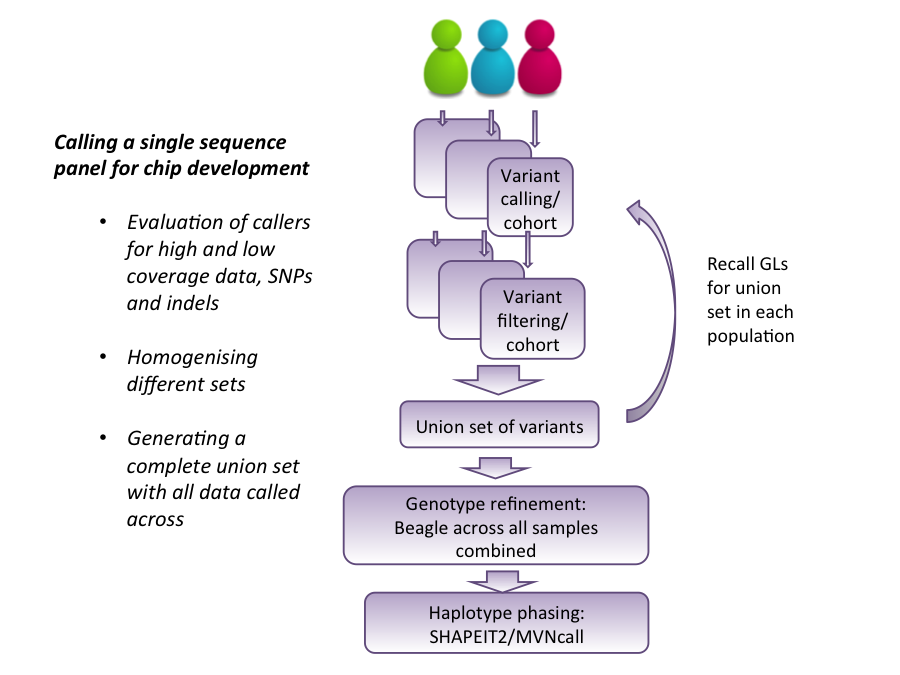
\includegraphics[width=0.8\textwidth]{calling}
\caption{Homogenised calling across all datasets to generate a single panel}
\label{fig:calling}
\end{figure}
%Datasets generated with unique Illumina chemistry, and those with different coverages will need to be called in separate subsets.
GATK3.3+ UnifiedGenotyper (UG) and GATK3.3+ HaplotypeCa ller (HC) will be used for calling SNPs from low and high coverage data, respectively. Multiple samples will be called simultaneously with UnifiedGenotyper, whereas HaplotypeCaller will be applied to individual samples in GVCF mode and subsequently joint genotyping will be carried out with GenotypeGVCFs. For compatibility reasons it is important that the same versions of HaplotypeCaller and GenotypeGVCFs are used.
%http://gatkforums.broadinstitute.org/discussion/5051/are-gatk-versions-3-compatible
During variant calling UG by default downsamples each sample randomly to a maximum coverage of 250 (\-\-downsampling\_type BY\_SAMPLE and \-\-downsample\_to\_coverage 250). We will use the default minimum base quality for UG, which is currently 17 (\-\-min\_base\_quality\_score 17). %10 for HC
At each site we don't call more than the 6 best alternate alleles (\-\-max\_alternate\_alleles 6).
For low coverage data we use calling and emission thresholds (\-stand\_call\_conf and \-stand\_emit\_conf) of 10 as the sample count is greater than 100 as per \href{https://www.broadinstitute.org/gatk/guide/pdfdocs/GATK_GuideBook_2.7-4.pdf}{GATK best practises}. %page 13
For high coverage data we use thresholds of 30 in accordance with GATK best practices.
%Indels will be called with a plethora of software packages (see the next section).

%If pedigree information is available, then this will be used by UnifiedGenotyper %and GenotypeGVCFs
%in calculation of the InbreedingCoeff annotation, which is used for subsequent variant filtering. Pedigree information will also be used for refinement and phasing. Incomplete pedigrees will be inferred from IBD matrices for sequenced and non-sequenced samples in each cohort.

%\subsubsection{Calling of short indels and structural variants}
With UG we will only make a call in the low coverage data, if the number of consensus indels exceeds a threshold of 5 (--min\_indel\_count\_for\_genotyping 5), which is the default value and the value used for phase 1 of 1000G.
%1000G low coverage indel calling by the Broad - "if a candidate indel allele was present in at least 5 reads at a site, it would be passed over to the next step for genotyping, or otherwise it was excluded."
We furthermore use PINDEL, GINDEL, Dindel, samtools, MATE-CLEVER and SOAPdenovo to call indels shorter than 100bp and deletions longer than 100bp. Breakdancer is used to identify structural variants (SVs) in trios. GenomeSTRiP is used for discovery of deletions. We will use best practices of each method to filter variants prior to creating a consensus set. For Pindel for example it will be a requirement that an indel appear in more than 3 samples and with more than 10 supporting reads in total among all samples.
%GoNL Indels (1-20bp) "GATK UG and at least one other algorithm"
%GoNL Deletions (20-100bp) "more than one method" "at least 3 families and transmitted to at least 1 child"
%GoNL Deletions (>100bp) "at least two algorithms" "at least 3 families and transmitted to at least 1 child"

We remove indels with the maximum number of alternate alleles.
%1000G called indels as biallelic.
Similar to 1000G we will remove protein-coding frameshift indels exclusive to low coverage samples and do post-hoc filtering of short indels with a support vector machine (SVM) or random forest (RF) machine learning approach and by applying a MAF threshold of 0.5\%. The latter machine learning method has been used successfully at the Broad Institute. One could classify indels by:
\begin{enumerate}
\item length (continuous or classified)
\item type (homopolymer run (HR) with runs of 6 or more identical nucleotides, tandem repeat (TR))
\item frameshift/nonframeshift in coding regions
\item tandem repeat length (dinucleotide repeat, trinucleotide repeat, STR/microsatellite (2-5/6/9), minisatellite (10-60)
%INSERTION-DELETION VARIANTS IN 179 HUMAN GENOMES - Table 3 - Characteristics of indels
\item HR insertion (more likely), HR deletion (less likely)
\item tandem repeat type (CG, non-CG)
\item SNP at same site, no SNP at same site
\item biallelic, multialleic
\item inside/outside RepeatMasker regions
\item P site / non-P site; i.e. the reference base not N, depth not less than half of average, depth not twice of average, less than 20\% of reads at position have MQ of 0, base not covered. Calculate averages for the autosomes and the X chromosome independently.
\item allele balance
\item strand bias
\item mapping quality
\item number of supporting non-reference reads
\item distance to nearby indels
\item cytoband: gneg, gpos25, gpos50, gpos75, gpos100, acen, gvar
\end{enumerate}

The NIST NA12878 truth set currently does not hold information on structural variants (SVs). We therefore carry out calling of SVs with multiple callers, apply default calling thresholds and use a consensus dataset as the final SV dataset.

Other variant callers to consider are listed in the table below.
\begin{table}[h]
\centering
\resizebox{\textwidth}{!}{%
\begin{tabular}{|l|l|l|l|l|l|l|l|}
\hline
Name & Year & 1000G & GoNL & Method & de novo assembly & Length & Status \\ \hline
%http://homepages.cwi.nl/~as/software.html
%Mendelian-inheritance-aware discovery and genotyping of midsize and long indels
%.nl
MATE-CLEVER\cite{Marschall2013} & 2014 & & 1-20bp, 20-100bp, \textgreater100bp & read pair / split read  & 1-20bp & \\ \hline
%Pindel good according to ClipCrop paper
%"Pindel only works well for high coverage data, but does not perform well at low coverage." - GINDEL paper
%does Pindel report genotypes?
%http://gmt.genome.wustl.edu/packages/pindel/
Pindel\cite{Ye2009} & 2014 & SV \textgreater50bp & 1-20bp, 20-100bp, /textgreater100 (v0.2.4) & pattern growth? split read &  & 1bp- & Develop \\ \hline
%"Pindel only works well for high coverage data, but does not perform well at low coverage." - GINDEL paper
%"Genome STRiP performs less well for shorter deletions (50–200 bp)" - GINDEL paper
%http://www.engr.uconn.edu/~ywu/
GINDEL\cite{Chu2014GINDEL} & 2014 & No & No &  &  &  \\ \hline
%"Genome STRiP performs less well for shorter deletions (50–200 bp)" - GINDEL paper
%Support for accessing bam files over http, ftp and s3.
%http://www.broadinstitute.org/software/genomestrip/genome-strip
GenomeSTRiP & 2013 & SV \textgreater50bp & 1-20bp, 20-100bp, \textgreater100bp (v1.04.915) & read depth / read pair &  & \\ \hline
% Dindel sensitivity good for low coverage data according to Neuman2012
%https://www.sanger.ac.uk/resources/software/dindel/
Dindel2\cite{Albers01062011} & 2011 & indels & & Bayesian, short-read data & No & \textless50bp \\ \hline
%samtools emits left aligned INDELs
samtools\cite{Li2009} & 2014 & indels &  &  &  & & Develop \\ \hline
FreeBayes & 2014 & Yes &  & Larger INDELs with local assembly &  &  \\ \hline
%Platypus compared to GATK UG, HC and SAMtools
%Platypus emits left aligned INDELs
%evaluated on the high coverage NA12878 trio
%evlauated against fosmid data (ref26)
Platypus\cite{Rimmer2014} & 2014 & indels &  & Local assembly &  & Deletions\textgreater1kb, insertions~300bp & Develop \\ \hline
SOAPIndel/SOAPdenovo & 2014 & & 1-20bp, 20-100bp, \textgreater100bp & de novo assembly of unmapped reads with mapped partner & Yes & \textlessread length & Develop \\ \hline
%Cortex does not require prior mapping
Cortex\cite{Iqbal2012Cortex} & 2013 & Yes &  & reference-free sequence assembly & Yes, Global &  \\ \hline
%GATK emits left aligned INDELs
GATK HaplotypeCaller & 2014 & No & No & Local reassembly & Yes, Local & 1-100bp & Develop \\ \hline
123SV & 2011 & & 20-100bp, \textgreater100bp (v0.9) & read pair &  & \textgreater100bp \\ \hline
DWACSeq & & & \textgreater100bp (v0.7) & read depth based &  & \\ \hline
CNVnator & 2014 & SV \textgreater50bp & \textgreater100bp (v0.2.2) & depth of coverage approach &  & \textgreater window size (e.g. 100) \\ \hline
FACADE & &  & \textgreater100bp & read depth based &  & \\ \hline
%VarScan2.2.2 Not good according to Neuman2012 (figure 4)
%VarScan worse than Dindel (sens and FDR) according to Dindel paper
VarScan\cite{Koboldt01032012} & &  &  &  &  &  \\ \hline
%UG does poorly for low coverage data according to Neuman2012 (figure 4)
GATK UnifiedGenotyper & 2013 &  & 1-20bp, 20-100bp (2.1.8) &  &  & & Abandon  \\ \hline
%BreakDancer Not good according to ClipCrop paper
%Trios only! Used for trios in GoNL paper.
BreakDancer & & SV \textgreater50bp & 20-100bp, \textgreater100bp (v1.1) & Discordant/read pair approach &  & 20-100bp \\ \hline
ClipCrop & 2011 & &  &  &  & & Abandon \\ \hline
DELLY & & SV \textgreater50bp &  &  &  & & \\ \hline
\end{tabular}
}
\caption{Characteristics of INDEL callers. Year refers to latest release/update.}
\label{INDELcallers}
\end{table}

\subsubsection{Calling of chromosomes X and Y}
The X chromosome will be called jointly for males and females with the same ploidy, because the memory and CPU use of UG otherwise grows intensely. Likewise the pseudoautosomal regions (PARs) 1 and 2 on the X chromosome will be called like the autosomes; i.e. jointly for males and females with all samples treated as diploid. The Y chromosome will also be treated as diploid due to the UG memory and CPU issue, when doing haploid variant calling, but variant calling will only be carried out for males. The PARs on the Y chromosome are masked in the reference sequence and not subject to calling. An excessive number of heterezogyous calls of haploid genotypes can be utilized for a QC step of sites and samples; thresholds to be decided.
%The mitochondrial variants will be called with GATK, VarScan2\cite{Koboldt2012} and MitoSeek and the union set recalled and annotated with GATK prior to filtering. VarScan is chosen, because it performs well at extreme read depths.\cite{Stead2013} MitoSeek is a software package dedicated to calling variants from mtDNA reads. When calling with GATK the ploidy will be set to the mean coverage in the MT contig divided by the mean coverage in the somatic chromosomes.
%ftp://ftp.1000genomes.ebi.ac.uk/vol1/ftp/technical/reference/phase2_reference_assembly_sequence/README_human_reference_20110707
%http://gatkforums.broadinstitute.org/discussion/1214/can-i-use-gatk-on-non-diploid-organisms
%GoNL - "Consensus sequences were called by GATK."

%\begin{table}[h]
\centering
\begin{tabular}{l|l|l|}
\cline{2-3}
\rowcolor[HTML]{FFFFFF} 
                          & Male & Female \\ \hline
\multicolumn{1}{|l|}{X}   & 1    & 2      \\ \hline
\multicolumn{1}{|l|}{Y}   & 1    & N/A    \\ \hline
\multicolumn{1}{|l|}{PAR} & 2    & 2      \\ \hline 
\end{tabular}
\caption{Ploidies used for calling variants on the sex chromosomes.}
\label{table:XYcalling}
\end{table}
